\RequirePackage{ifpdf}
\documentclass[a4paper,11pt]{article}
\usepackage{pgfplots,tocloft}
\pgfplotsset{width=7cm,compat=1.9}
%--This is to improve loading time
\usepgfplotslibrary{external}
\tikzexternalize
%--This is the end!
\renewcommand{\cftsecfont}{\normalfont}
\renewcommand{\cftsecpagefont}{\normalfont}
\renewcommand{\cftsecleader}{\cftdotfill{\cftsecdotsep}}
\renewcommand{\cftsecdotsep}{\cftdot}
\renewcommand{\cftsubsecdotsep}{\cftdot}
\renewcommand\cftsecaftersnum{.}
\renewcommand\thesection{\Roman{section}}
\author{Son To}
\date{June 13th, 2017}
\title{PGFPlot-A simple tutorial\footnote{This
tutorial is taken from
\href{https://www.sharelatex.com/learn/Pgfplots_package#/The_document_preamble}{this link}
with some modifications for personal pleasure!}}
\usepackage[pdftex,hyperindex=false,colorlinks,%
bookmarks,unicode]{hyperref}
\ifpdf
  \hypersetup{linkcolor=blue}
\else
  \hypersetup{linkcolor=black}
\fi
\begin{document}
  \maketitle
  \tableofcontents
  \clearpage
  \section{The Basic}
  Pgfplots is a powerful package specialized in creating
  powerful scientific \nolinebreak graphs.
  \begin{tikzpicture}
    \begin{axis}
      \addplot[color=blue]{exp(x)};
    \end{axis}
  \end{tikzpicture}
  % Here ends the first plot.
  \hskip 5pt
  % Here starts the 3d plot.
  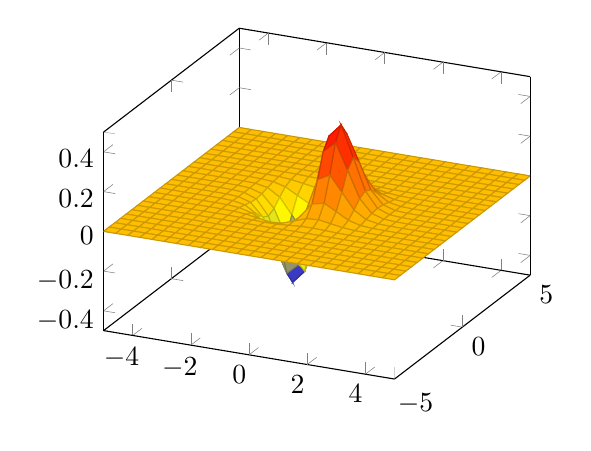
\begin{tikzpicture}
    \begin{axis}
      \addplot3[
      surf,
      ]{exp(-x^2-y^2)*x};
    \end{axis}
  \end{tikzpicture}
We now get to some more details on 2D plot.
\clearpage
\section{2D Plot}
What the heck...Let's do some damage!

\begin{tikzpicture}
  \begin{axis}[
    axis lines= center,
    xlabel= $x$,
    ylabel= {$f(x)$},
    legend style={at={(axis cs:10,5)},anchor=north east},
    ]
    %We now add a red parabola
    \addplot[
    domain=-10:10,
    samples=100,
    color=red,
    ]
    {x^2-2*x-1};
    \addlegendentry{$x^2-2x-1$}
    %Now we add another parabola to the same axis
    \addplot[
    domain=-10:10,
    samples=100,
    color=blue
    ]
  \end{axis}
\end{tikzpicture}
Come on man!!!!
\end{document}
